
The process of scientific discovery, as explained by Richard Feynman, usually starts with guesses.
The consequences of such guesses are then computed and compared with experimental results.
If the predictions disagree with the experiment then our guesses are wrong. ``That is all there is to it''  \citep{feynman2017character}.

In the previous chapters, we delved deep into the theoretical underpinnings of the phase transition phenomena in high-dimensional multiple testing problems.
The results are interesting in their own right.
However, we have not discovered any scientific law in the spirit of Feynman, but merely worked out mathematical consequences of our postulated models.
In this chapter, our goal is to relate these predictions to real experimental data from the field of genetics, where large-scale simultaneous hypotheses testing problems often arise.
From such comparisons, we will demonstrate that the phase transition laws are indeed reasonable predictions of some curious phenomena in that field.
The accuracy of our predictions will lend credibility to the application of these ``laws of large dimensions'' in actual applications.

\medskip

In our case, the experimental data used as the measuring stick come from genome-wide association studies (\ac{GWAS}), introduced in Section \ref{sec:motivation-chisq}.
Recall that in \ac{GWAS}, a large number of marginal association tests are conducted simultaneously, resulting in statistics that can be approximated by
\begin{equation} \label{eq:model-chisq-Chapter6}
    %x(i) \distras{\mathrm{ind.}} \chi_\nu^2\left(\lambda(i)\right), \quad i=1,\ldots,p.
    x(i) \sim \chi_\nu^2\left(\lambda(i)\right), \quad i=1,\ldots,p,
\end{equation}
where $\chi_\nu^2\left(\lambda(i)\right)$ is a chi-square distributed random variable with $\nu>0$ degrees of 
freedom\footnote{The parameter $\nu$ here should not be confused with the shape parameter of the AGG$(\nu)$ 
distributions, which will not appear in this chapter.} and non-centrality parameter $\lambda(i)$.


We establish our theoretical predictions in two steps.
In Section \ref{sec:chisq-boundaries} below, we shall first establish the phase transitions of the model \eqref{eq:model-chisq-Chapter6}.
In parallel to results in Chapter \ref{chap:phase-transitions}, we show that several commonly used family-wise error rate-control procedures --- including Bonferroni's procedure --- are asymptotically optimal for the {exact}, and {exact-approximate} support recovery problems (recall Definition \ref{def:exact-recovery-success-failure}) in idealized chi-square models with independent components.
Analogously, the \ac{BH} procedure is asymptotically optimal for the {approximate}, and {approximate-exact} support recovery problems.
% \ref{thm:chi-squared-exact-boundary}, \ref{thm:chi-squared-exact-approx-boundary}, \ref{thm:chi-squared-approx-boundary}, and \ref{thm:chi-squared-approx-exact-boundary}.
Under appropriate parametrization of the signal sizes and sparsity, we establish the phase transitions of support recovery problems in the chi-square model.
Remarkably, the degree-of-freedom parameter does not affect the asymptotic boundaries in any of the four support recovery problems.

In the second step, we translate the canonical signal size and sparsity parametrizations into the vernacular of statistical geneticists in Section \ref{sec:odds-and-power}.
% present empirical evidence for the phase transition in the exact-approximate problem using real data from large-scale association studies on breast cancer obtained from the NHGRI-EBI GWAS Catalog \citep{macarthur2016new}.
% demystify the notion of signal size $\lambda$ in this context.
% which is perhaps less transparent than in additive error models.
We do so by characterizing the relationship between the signal size $\lambda$ and the marginal frequencies, odds ratio, and sample sizes for association tests on 2-by-2 contingency tables. 
This is important because these parameters are often estimated and reported in \ac{GWAS}, while we have never seen the elusive signal size parameter $\lambda$ reported.
% Specifically, the amount of signal, when rare variants are present, is weaker compared to the signal when the marginal distributions are balanced.
% In other words, reliable detection of the effects by rare variants would require more samples compared to common variants, even at the same odds ratio.
% This result, establishing the relationship between sample sizes and signal sizes, is made precise in Section \ref{sec:odds-and-power}.
As a bonus, we point out the implications of this relationship on statistically optimal study designs for association studies in Section \ref{sec:optimal-design}:
perhaps surprisingly, balanced designs with equal number of cases and controls are often statistically inefficient.
% Practical consequences of these results in power analysis will be illustrated with data examples in Section \ref{sec:phase-transitions-in-GWAS}. 

Armed with the results on phase transitions in the chi-square model, and a translation from the language of high-dimenstional statistics to the patois of association screening studies, we finally present in Section \ref{sec:phase-transitions-in-GWAS} the consequences of the phase transitions in \ac{GWAS}, and compare against real experimental data to evaluate the success of our predictions.

The phase transitions in the chi-square models are demonstrated with numerical simulations in Section \ref{sec:numerical}.
The proofs, which are closely resemble those of the results in Chapter \ref{chap:phase-transitions}, are collected in Section \ref{sec:supplement:proofs}.
%in Section \ref{sec:proof-signal-size-odds-ratio}.

% Practical issues are also addressed to make for simple and effective power analysis.

\section{Support recovery problems in chi-squared models}
\label{sec:chisq-boundaries}

Similar to the analysis of additive error models in Chapter \ref{chap:phase-transitions}, we will work with triangular arrays of chi-square models \eqref{eq:model-chisq-Chapter6} indexed by $p$.
We adopt the same parametrization for the sparsity of the non-centrality parameter vectors $\lambda = \lambda_p$,
\begin{equation} \label{eq:signal-sparsity}
    |S_p| = \left\lfloor p^{1-\beta} \right\rfloor, \quad \beta\in(0,1]
\end{equation}
where $S_p:= \{ i\, :\, \lambda(i) >0 \}$ is the {\em signal support} set and  $\beta$ parametrizes the problem {\em sparsity}.
The closer $\beta$ is to 1, the sparser the support $S_p$; conversely, when $\beta$ is close to 0, the support is dense with many non-null signals.

We parametrize the range of the non-zero and perhaps unequal signals in the chi-square model with
\begin{equation} \label{eq:signal-size}
    \underline{\Delta} = 2\underline{r}\log{p}
    \le \lambda(i) \le
    \overline{\Delta} = 2\overline{r}\log{p}, \quad \text{for all}\;\;i\in S_p,
\end{equation}
for some constants $0<\underline{r}\le\overline{r}\le+\infty$.

\subsection{The exact support recovery problem}
\label{subsec:exact-support-recovery-chisq}

The first main result characterizes the phase transition phenomenon in the exact support recovery problem under the chi-square model.  It parallels
Theorem \ref{thm:Gaussian-error-exact-boundary}.

\begin{theorem} \label{thm:chi-squared-exact-boundary}
Consider the high-dimensional chi-squared model \eqref{eq:model-chisq-Chapter6} with signal sparsity and size as described in \eqref{eq:signal-sparsity} and \eqref{eq:signal-size}.
The function 
\begin{equation} \label{eq:exact-boundary-chisquared}
    f_{\mathrm{E}}(\beta) = \left(1 + \sqrt{1-\beta}\right)^2
\end{equation}
characterizes the phase transition of exact support recovery problem.
Namely, the following two results hold.\\

{\rm (i)} If $\underline{r} > f_{\mathrm{E}}(\beta)$, then Bonferroni's, Sid\'ak's, Holm's, and Hochberg's procedures with slowly vanishing (see Definition \ref{def:slowly-vanishing}) nominal FWER levels all achieve asymptotically exact support recovery in the sense of \eqref{eq:support-recovery-success}.\\

{\rm (ii)} Conversely, if $\overline{r} < f_{\mathrm{E}}(\beta)$, then for any thresholding procedure $\widehat{S}_p$, we have $\P[\widehat{S}_p=S_p]\to0$.
Therefore, in view of Lemma \ref{lemma:risk-exact-recovery-probability}, exact support recovery asymptotically fails for all thresholding procedures in the sense of \eqref{eq:support-recovery-failure}.
\end{theorem}

% \begin{figure}
%   \begin{center}
%     \includegraphics[width=0.7\textwidth]{./pics/phase_diagram_chisquared_ALL_boundaries.eps}
%   \end{center}
%    \caption{The phase diagram for the high-dimensional chi-square model \eqref{eq:model-chisq}, illustrating the boundaries of the exact support recovery (FWER + FWNR; top curve; Theorem \ref{thm:chi-squared-exact-boundary}), the approximate-exact support recovery (FDR + FWNR; second curve from top; Theorem \ref{thm:chi-squared-approx-exact-boundary}), the exact-approximate support recovery (FWER + FNR; horizontal line $r=1$; Theorem \ref{thm:chi-squared-exact-approx-boundary}), and the approximate support recovery problems (FDR + FNR; tilted line $r=\beta$; Theorem \ref{thm:chi-squared-approx-boundary}). The signal detection problem (type I + type II errors of the global test; lower curve) was studied in Donoho and Jin (2004). In each region of the diagram and above, the annotated statistical risk can be made to vanish, as dimension $p$ diverges. Conversely, the risks has liminf at least one. All boundaries are unaffected by the degree-of-freedom. All boundaries are identical to those in the Gaussian additive error model \eqref{eq:model-additive} under one-side alternatives; c.f., results in Section \ref{sec:additive-error-model-boundaries}.}
%    \label{fig:phase-chi-squared}
% \end{figure}


The procedures listed in Theorem \ref{thm:chi-squared-exact-boundary} were reviewed in Section \ref{sec:statistical-procedures}. 
The proof of the theorem can be found in Section \ref{subsec:proof-chi-squared-exact-boundary}. 
% The boundary \eqref{eq:exact-boundary-chisquared} is plotted in Figure \ref{fig:phase-chi-squared}.

It is evident that the exact support recovery boundary \eqref{eq:exact-boundary-chisquared} coincides with that in parallel results for the Gaussian additive error models \eqref{eq:model-additive} in Chapter \ref{chap:phase-transitions}.
Implications of these results will be discussed in Section \ref{subsec:one-vs-two-sided} below.

\begin{remark} \label{rmk:strong-classification-boundary-2}
Theorem \ref{thm:chi-squared-exact-boundary} predicts that the asymptotic boundaries are the same for all values of the degrees of freedom 
parameter $\nu$.  In simulations (Section \ref{sec:numerical}), we find this asymptotic prediction to be quite accurate for $\nu\le3$ even in 
moderate dimensions ($p=100$).  For $\nu>3$, the phase transitions take place somewhat above the boundary ${g}$.
The behavior is qualitatively similar for the other three phase transitions (see Theorems \ref{thm:chi-squared-exact-approx-boundary}, 
\ref{thm:chi-squared-approx-boundary}, and \ref{thm:chi-squared-approx-exact-boundary} below).
\end{remark}

\subsection{The exact-approximate support recovery problem}
\label{subsec:exact-approx-support-recovery-chisq}

The next theorem describes the phase transition in the exact-approximate support recovery problem. Recall also
Theorem \ref{thm:Gaussian-error-exact-approx-boundary}.

\begin{theorem} \label{thm:chi-squared-exact-approx-boundary}
In the context of Theorem \ref{thm:chi-squared-exact-boundary}, 
the function 
\begin{equation} \label{eq:exact-approx-boundary-chisquared}
    f_{\mathrm{EA}}(\beta) = 1
\end{equation}
characterizes the phase transition of exact-approximate support recovery problem.
 Namely, the following two results hold.\\

{\rm (i)} If $\underline{r} > f_{\mathrm{EA}}(\beta)$, then the procedures listed in Theorem \ref{thm:chi-squared-exact-boundary} with slowly 
vanishing nominal FWER levels achieve asymptotically exact-approximate support recovery in the sense of \eqref{eq:support-recovery-success}. \\

{\rm (ii)} Conversely, if $\overline{r} < f_{\mathrm{EA}}(\beta)$, then for any thresholding procedure $\widehat{S}_p$, the exact-approximate support recovery fails in the sense of \eqref{eq:support-recovery-failure}.
\end{theorem}

Theorem \ref{thm:chi-squared-exact-approx-boundary} is proved in Section \ref{subsec:proof-chi-squared-mix-boundaries}. 


\subsection{The approximate support recovery problem}
\label{subsec:approx-support-recovery-chisq}

Our third asymptotic result characterizes the phase transition phenomenon in the approximate support recovery problem in the chi-square model.
It closely parallels Theorem \ref{thm:Gaussian-error-approx-boundary} for the additive errors model.

\begin{theorem} \label{thm:chi-squared-approx-boundary}
Consider the high-dimensional chi-squared model \eqref{eq:model-chisq-Chapter6} with signal sparsity and size as described in \eqref{eq:signal-sparsity} and \eqref{eq:signal-size}.
The function 
\begin{equation} \label{eq:approx-boundary-chisquared}
    f_{\mathrm{A}}(\beta) = \beta
\end{equation}
characterizes the phase transition of approximate support recovery problem. Specifically the following two results hold.\\

{\rm (i)} If $\underline{r} > f_{\mathrm{A}}(\beta)$, then the \ac{BH} procedure $\widehat{S}_p$ (defined in Section \ref{sec:statistical-procedures}) with slowly vanishing (see Definition \ref{def:slowly-vanishing}) nominal FDR levels achieves asymptotically approximate support recovery in the sense of \eqref{eq:support-recovery-success}. \\

{\rm (ii)} Conversely, if $\overline{r} < f_{\mathrm{A}}(\beta)$, then approximate support recovery asymptotically fails in the sense of \eqref{eq:support-recovery-failure} for all thresholding procedures.
\end{theorem}

Theorem \ref{thm:chi-squared-approx-boundary} is proved in Section \ref{subsec:proof-chi-squared-mix-boundaries} below. 


\subsection{The approximate-exact support recovery problem}
\label{subsec:aprox-exact-support-recovery-chisq}

A counterpart of Theorem \ref{thm:Gaussian-error-approx-exact-boundary} also holds in the chi-square models.

\begin{theorem} \label{thm:chi-squared-approx-exact-boundary}
In the context of Theorem \ref{thm:chi-squared-approx-boundary}, the function 
\begin{equation} \label{eq:approx-exact-boundary-chisquared}
    f_{\mathrm{AE}}(\beta) = \left(\sqrt{\beta} + \sqrt{1-\beta}\right)^2
\end{equation}
characterizes the phase transition of approximate-exact support recovery problem. Namely, 
the following two results hold.\\

{\rm (i)} If $\underline{r} > f_{\mathrm{AE}}(\beta)$, then the Benjamini-Hochberg procedure with slowly vanishing nominal FDR levels achieves asymptotically approximate-exact support recovery in the sense of \eqref{eq:support-recovery-success}. \\

{\rm (ii)} Conversely, if $\overline{r} < f_{\mathrm{AE}}(\beta)$, then for any thresholding procedure $\widehat{S}_p$, the approximate-exact support recovery fails in the sense of \eqref{eq:support-recovery-failure}.
\end{theorem}

Theorem \ref{thm:chi-squared-approx-exact-boundary} is proved in Section \ref{subsec:proof-chi-squared-exact-boundary}. 

Notice that all phase transitions boundaries are identical to those in the Gaussian additive error model \eqref{eq:model-additive} under one-sided alternative.
We refer readers to Figure \ref{fig:phase-Gaussian-errors} in Section \ref{sec:additive-error-model-boundaries} for a visualization of the results in Theorems \ref{thm:chi-squared-exact-boundary} through \ref{thm:chi-squared-approx-exact-boundary}.

\medskip

All four phase transitions results in Theorems \ref{thm:chi-squared-exact-boundary} through \ref{thm:chi-squared-approx-exact-boundary} 
focus only on the idealized models \eqref{eq:model-chisq-Chapter6} where the statistics are \emph{independent}.
Support recovery problems under dependent observations remain to be explored.
Recall in Chapter \ref{chap:exact-support-recovery} we showed that the boundary for the exact support recovery problem in the additive error model 
\eqref{eq:model-additive} continues to hold even under {\em severe dependence} and general distributional assumptions.
We conjecture that the concentration of maxima phenomenon, which is at the heart of the results in Chapter \ref{chap:exact-support-recovery}, will play
a role and all of the above phase-transition results will continue to hold, under broad dependence conditions in the chi-square models. As an example, 
in the GWAS application, dependence among the genetic markers at different locations (known as linkage disequilibrium) decay as a function of their physical distances on the genome \citep{bush2012genome}, resulting in locally dependent test statistics.
It would be of great interest to extend the current theory to cover important dependence structures that arise in such applications.


\subsection{Comparison of one- versus two-sided alternatives in additive error models}
\label{subsec:one-vs-two-sided}


% $\mathrm{risk}^{\mathrm{EA}}$ and $\mathrm{risk}^{\mathrm{AE}}$.
As alluded to in Chapter \ref{sec:motivation-chisq} in the introduction, we draw explicit comparisons between the one-sided and two-sided alternatives in Gaussian additive error models \eqref{eq:model-additive}.
% The exact, and the approximate support recovery problems in the additive error model \eqref{eq:model-additive} under standard Gaussian errors have been studied in \cite{gao2018fundamental} and \cite{arias2017distribution}, respectively. 

The exact support recovery problem in the dependent Gaussian additive error model \eqref{eq:model-additive} was studied in Chapter \ref{chap:phase-transitions}, with parametrization of sparsity identical to that in \eqref{eq:signal-sparsity}, whereas the range of the non-zero (and perhaps unequal) mean shifts $\mu(i)$ was parametrized as 
\begin{equation*}
    \underline{\Delta} = \sqrt{2\underline{r}\log{p}}
    \le \mu(i) \le
    \overline{\Delta} = \sqrt{2\overline{r}\log{p}}, \quad \text{for all}\;\;i\in S_p,
\end{equation*}
for some constants $0<\underline{r}\le\overline{r}\le+\infty$.
Under this one-sided alternative, a phase transition in the $r$-$\beta$ plane was described, where the boundary was found to be identical to \eqref{eq:exact-boundary-chisquared} in Theorem \ref{thm:chi-squared-exact-boundary} for the chi-square models \eqref{eq:model-chisq-Chapter6}. 

As discussed in Section \ref{sec:motivation-chisq}, support recovery problems in the chi-square model with $\nu=1$ correspond to the support recovery problems in 
the additive model under two-sided alternatives. This implies that the asymptotic signal size requirements are identical between the two-sided alternative and its 
one-sided counterpart, in order to achieve exact support recovery. As we shall see in numerical experiments (in Section \ref{sec:numerical} below), the difference 
is not very pronounced even in moderate dimensions, and vanishes as $p\to\infty$, in accordance with Theorem \ref{thm:chi-squared-exact-boundary}.

\medskip

Comparisons can also be drawn in the approximate, approximate-exact, and exact approximate support recovery problems between the two types of alternatives.

Specifically, the approximate support recovery problem in the Gaussian additive error model \eqref{eq:model-additive} under one-sided alternatives exhibits a phase transition phenomenon characterized by a boundary that coincides with \eqref{eq:approx-boundary-chisquared} in Theorem \ref{thm:chi-squared-approx-boundary}.
Similar to the exact support recovery problem, this indicates vanishing difference in the difficulties of the two types alternatives in approximate support recovery problems.

Comparing Theorems \ref{thm:chi-squared-exact-approx-boundary} and \ref{thm:Gaussian-error-exact-approx-boundary} as well as
 Theorems \ref{thm:chi-squared-approx-exact-boundary} and \ref{thm:Gaussian-error-approx-exact-boundary}, we see that the phase transition boundaries under the two types of alternatives are also identical in the exact-approximate and approximate-exact support recovery problems.

To complete the comparisons, we point out that the phase transition boundaries for the sparse signal {detection} problem in the two types of alternatives are both identical to \eqref{eq:detection-boundary-large-signals}. This was analyzed in \cite{donoho2004higher}.

Therefore, all phase transition boundaries coincide with those in the additive error models obtained in Chapter \ref{chap:phase-transitions} under their respective parametrizations.
% and Figure \ref{fig:phase-chi-squared} continues to apply.
This indicates vanishing differences between the difficulties of the one-sided and two-sided alternatives in the Gaussian additive error model 
\eqref{eq:model-additive}. The additional uncertainty in the two-sided alternatives does not call for larger signal sizes in these problems, asymptotically.





\section{Odds ratios and statistical power}
\label{sec:odds-and-power}

We return to the application of association screenings for categorical variables, and put the results in the previous section to use.
In particular, we focus on the exact-approximate support recovery problem, and demonstrate the consequences of its phase transition (Theorem \ref{thm:chi-squared-exact-approx-boundary}) in genetic association studies.

In order to do so, we must first connect the concept of statistical signal size $\lambda$ with some key quantities in association tests.
While the term ``signal size'' likely sounds foreign to most practitioners, it is intimately linked with the concept of ``effect sizes'' --- or odds ratios --- in association studies, which are frequently estimated and reported in GWAS catalogs. 
Effect sizes, on the other hand, may be alien to some statisticians.  
In this section, we aim to bridge the two languages by characterizing the relationship between ``signal size'' and ``odds-ratio'' parameterizations in the special, but fairly common case of association tests on 2-by-2 contingency tables.

 %in Section \ref{sec:odds-and-power}.

% Unlike in additive models where the parameter $\mu$ has the interpretation of signal-to-noise ratios, the meaning of the signal sizes $\lambda$ in chi-square model is perhaps not as transparent.

Recall the general setup of genetic association testing in Section \ref{sec:motivation-chisq}, where one wants to detect the association between genetic variations at a specific location and the occurrence of a disease. 
An individual randomly drawn from the target population will have two (random) characteristics: a phenotype indicating whether the individual has the condition or is healthy (i.e., belonging to the Case group or the Control group), and a genotype that encodes the genetic variation in question. 
Table \ref{tab:multinomial-counts} in the introduction summarizes the {\em counts} for all phenotype-genotype combinations for the individuals in a given study sampled from the population.
These counts may be assumed to follow a multinomial distribution, with probabilities given in Table \ref{tab:multinomial-probabilites} below. 
% Notice that there are fundamental study design questions here since the counts will depend on the way individuals are recruited in the study. 
% For example, ``controlling'' the number of Cases or Controls (as opposed to sampling at random from the population) will change the theoretical parameters (probabilities) of the multinomial model.
% These questions will be addressed in Section \ref{sec:optimal-design} below.

Consider a 2-by-2 multinomial distribution with marginal probabilities of phenotypes $(\phi_1, \phi_2)$ and genotypes $(\theta_1, \theta_2)$.
The \emph{probability} table (as opposed to the table of multinomial \emph{counts} in the introduction) is as follows.
\begin{table}[h]\label{tab:multinomial-probabilites}
\begin{center}
    \begin{tabular}{cccc}
    \hline
    & \multicolumn{2}{c}{Genotype} \\
    \cline{2-3}
    Probabilities & Variant 1 & Variant 2 & Total by phenotype \\
    \hline
    Cases & $\mu_{11}$ & $\mu_{12}$ & $\phi_1$ \\
    Controls & $\mu_{21}$ & $\mu_{22}$ & $\phi_2$ \\
    Total by genotype & $\theta_1$ & $\theta_2$ & 1 \\
    \hline
    \end{tabular}
    \caption{Probabilities of the multinomial distribution in a genetic association test. (Compare and contrast with 
    Table \ref{tab:multinomial-counts}. We have $\E[ O_{ij}] = n\mu_{ij},\ i,j=1,2$, where $n = \sum_{i,j} O_{ij}$.) }
\end{center}
\end{table}

The odds ratio (i.e., ``effect size'') is defined as the ratio of the phenotype frequencies between the two genotype variants,
\begin{equation} \label{eq:odds-ratio}
    \text{R} := \frac{\mu_{11}}{\mu_{21}}\Big/\frac{\mu_{12}}{\mu_{22}}
    = \frac{\mu_{11}\mu_{22}}{\mu_{12}\mu_{21}}.
\end{equation}
The multinomial distribution is fully parametrized by the trio $(\theta_1, \phi_1, R)$.
Odds ratios further away from 1 indicate greater contrasts between the probability of outcomes.
Independence between the genotypes and phenotypes would imply an odds ratio of one, and hence $\mu_{jk} = \phi_j\theta_k$, for all $j,k \in\{1,2\}$.

% When data are sampled from the multinomial distribution, the chi-square test defined in \eqref{eq:chisq-statistic} is asymptotically equivalent to tests including, e.g., the likelihood ratio test and Welch's t-test, both in terms of level and power \cite{ferguson2017course,gao2019upass}.
For a sequence of local alternatives $\mu^{(1)}, \mu^{(2)}, \ldots$, such that $\sqrt{n}(\mu^{(n)}_{jk} - \phi_j\theta_k)$ converges to a constant table $\delta = (\delta_{jk})$, the chi-square test statistics converge in distribution to the non-central chi-squared distribution with non-centrality parameter 
\begin{equation*}
    \lambda = \sum_{j=1}^2 \sum_{k=1}^2 {\delta_{jk}^2}/{(\phi_j\theta_k)}.
\end{equation*}
See, e.g., \cite{ferguson2017course}.
Hence, for large samples from a fixed distribution $(\mu_{ij})$, the statistic is well approximated by a $\chi^2_1(\lambda)$ distribution, where
\begin{equation} 
\lambda = n\sum_{j=1}^2 \sum_{k=1}^2 \frac{(\mu_{jk} - \phi_j\theta_k)^2}{\phi_j\theta_k}.
\end{equation}
%Since $\lambda$ is linear in the number of samples $n$, 
% Power of association tests at $\alpha$ level is approximately $\P[\chi^2_{\nu}(\lambda)>\chi^2_{\nu,\alpha}]$, where $\chi^2_{\nu,\alpha}$ is the upper $\alpha$-quantile of a central Chi-squared distribution.
Power calculations therefore only depend on the $\mu_{jk}$'s through $\lambda=nw^2$, where we define 
\begin{equation} \label{eq:signal-size-chisq}
    w^2:=\lambda/n
\end{equation} 
to be the \emph{signal size per sample}. 
Statistical power would be increasing in $w^2$ for fixed sample sizes.

The next proposition states that the statistical signal size per sample can be parametrized by the odds ratio and the marginals in the probability table.

\begin{proposition} \label{prop:signal-size-odds-ratio}
Consider a 2-by-2 multinomial distribution with marginal distributions $(\phi_1, \phi_2 = 1-\phi_2)$ and $(\theta_1, \theta_2=1-\theta_1)$.
Let signal size $w^2$ be defined as in \eqref{eq:signal-size-chisq}, and odds ratio $\text{R}$ be defined as in \eqref{eq:odds-ratio}. 
If $R=1$, we have $w^2 = 0$; if $R\in(0,1)\cup(1,+\infty)$, then we have
\begin{equation} \label{eq:signal-size-odds-ratio}
    w^2(\text{R}) =
    \frac{1}{4A(\text{R}-1)^2}\left(B+CR-\sqrt{(B+CR)^2-4A(R-1)^2}\right)^2,
\end{equation}
where $A = \phi_1\theta_1\phi_2\theta_2$, $B = \phi_1\theta_1+\phi_2\theta_2$, and $C = \phi_1\theta_2+\phi_2\theta_1$.
\end{proposition}

\begin{proof}
	We parametrize the 2-by-2 multinomial distribution with the parameter $\delta$, 
	\begin{equation} \label{eq:reparametrize-2-by-2-table-1}
	\mu_{11} = \phi_1\theta_1+\delta,\quad 
	\mu_{12} = \phi_1\theta_2-\delta,\quad 
	\mu_{21} = \phi_2\theta_1-\delta,\quad 
	\mu_{22} = \phi_2\theta_2+\delta.
	\end{equation}
	By relabelling of categories, we may assume $0<\theta_1,\phi_1\le1/2$ without loss of generality.
	Note that $\delta$ must lie within the range $[\delta_\mathrm{min}, \delta_\mathrm{max}]$, where
	$$
	\delta_\mathrm{min} := \max\{-\phi_1\theta_1, -\phi_2\theta_2, \phi_1\theta_2-1, \phi_2\theta_1-1\} 
	= -\phi_1\theta_1,
	$$
	and
	$$
	\delta_\mathrm{max} := \min\{1-\phi_1\theta_1, 1-\phi_2\theta_2, \phi_1\theta_2, \phi_2\theta_1\}
	= \min\{\phi_1\theta_2, \phi_2\theta_1\},
	$$
	in order for $\mu_{ij}\ge0$ for all $i,j\in \{1,2\}$.
	Under this parametrization, Relation \eqref{eq:odds-ratio} then becomes
	\begin{align} \label{eq:odds-ratio-delta}
	\text{R} = \frac{\mu_{11}\mu_{22}}{\mu_{12}\mu_{21}}
	= \frac{\phi_1\theta_1\phi_2\theta_2 + \delta(\phi_1\theta_1+\phi_2\theta_2)+\delta^2}{\phi_1\theta_1\phi_2\theta_2 - \delta(\phi_1\theta_2+\phi_2\theta_1)+\delta^2}
	= \frac{A +\delta B + \delta^2}{A -\delta C + \delta^2},
	\end{align}
	which is one-to-one and increasing in $\delta$ on $(\delta_\mathrm{min}, \delta_\mathrm{max})$.
	Equation \eqref{eq:signal-size-chisq} becomes
	\begin{equation} \label{eq:signal-size-chisq-delta}
	w^2 = \sum_{i=1}^2 \sum_{j=1}^2 \frac{(\mu_{ij} - \phi_i\theta_j)^2}{\phi_i\theta_j}
	= \delta^2\sum_i\sum_j \frac{1}{\phi_i\theta_j}
	= \frac{\delta^2}{\phi_1\theta_1\phi_2\theta_2},
	\end{equation}
	Solving for $\delta$ in \eqref{eq:odds-ratio-delta}, and plugging into the expression for signal size \eqref{eq:signal-size-chisq-delta} yields Relation \eqref{eq:signal-size-odds-ratio}.
	
	The other three cases ($1/2\le\theta_1,\phi_1\le1$; $0<\theta_1\le1/2\le\phi_1\le1$; and $0\le\phi_1\le1/2\le\theta_1\le1$) may be obtained similarly, or by appealing to the symmetry of the problem.
\end{proof}

To understand Proposition \ref{prop:signal-size-odds-ratio}, we illustrate Relation \eqref{eq:signal-size-odds-ratio} for selected values of marginals $\theta_1$ and $\phi_1$ in Figure \ref{fig:signal-vs-odds}.
Observe in the figure that an odds ratio further away from one corresponds to stronger statistical signal per sample, ceteris paribus.
However, this ``valley'' pattern is in general not symmetric around 1, except for balanced marginal distributions ($\phi_1=1/2$ or $\theta_1=1/2$).
While the odds ratio $R$ can be arbitrarily close to 0 or diverge to $+\infty$ for any marginal distribution, the signal sizes $w^2$ are bounded from above by constants that depend only on the marginals.
% This is quantified in the next corollary.

\begin{figure}
      \centering
      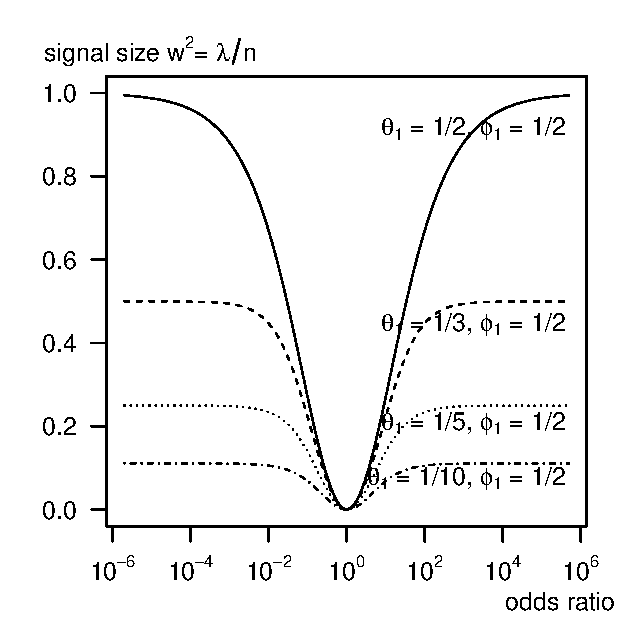
\includegraphics[width=0.49\textwidth]{pics/singal-vs-odds-p05}
      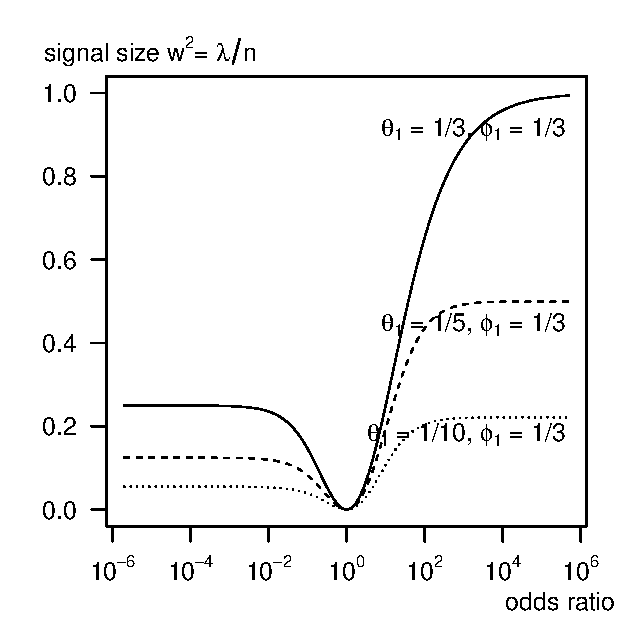
\includegraphics[width=0.49\textwidth]{pics/singal-vs-odds-p0333}            
      \caption{Signal sizes per sample $w^2$ as functions of odds ratios in 2-by-2 multinomial distributions for selected genotype marginals in balanced (left) and unbalanced (right) designs; see Relation \eqref{eq:signal-size-odds-ratio} in Proposition \ref{prop:signal-size-odds-ratio}. For given marginal distributions, extreme odds ratios imply stronger statistical signals at a given sample size. However, the signal sizes are bounded above by constants that depend on the marginal distributions; see Relations \eqref{eq:signal-size-upper-bound-1} and \eqref{eq:signal-size-upper-bound-2}. % Unbalanced marginal distributions -- or rare variants -- lead to smaller signal sizes at a given odds ratio.
      } 
      \label{fig:signal-vs-odds}
\end{figure}

\begin{corollary} \label{cor:signal-limits-OR}
The signal size as a function of the odds ratio $w^2(R)$ is decreasing on $(0,1)$ and increasing on $(1,\infty)$, with limits
\begin{equation} \label{eq:signal-size-upper-bound-1}
    \lim_{\text{R}\to0_+} w^2(\text{R}) = \min\left\{\frac{\phi_1\theta_1}{\phi_2\theta_2}, \frac{\phi_2\theta_2}{\phi_1\theta_1}\right\},
\end{equation}
and
\begin{equation} \label{eq:signal-size-upper-bound-2}
    \lim_{\text{R}\to+\infty} w^2(\text{R}) = \min\left\{\frac{\phi_1\theta_2}{\phi_2\theta_1}, \frac{\phi_2\theta_1}{\phi_1\theta_2}\right\}.
\end{equation}
\end{corollary}
% Proof of Corollary \ref{cor:signal-limits-OR} is found in Appendix \ref{sec:proof-signal-size-odds-ratio}. 

\begin{proof}
	As in the proof of Proposition \ref{prop:signal-size-odds-ratio}, we examine the case where $0<\theta_1,\phi_1\le1/2$, and leave the other three cases an exercise.
	Take the first derivative of the expression for $w^2$ in equation \eqref{eq:signal-size-chisq-delta} with respect to $\delta$, it is evident that $w^2(\delta)$ is decreasing on $[\delta_\mathrm{min},0)$, increasing on $(0,\delta_\mathrm{max}]$, with limits
	$$
	\lim_{d\to \delta_\mathrm{min}} w^2(\delta) = \frac{\phi_1\theta_1}{\phi_2\theta_2},
	\quad
	\text{and}
	\quad
	\lim_{d\to \delta_\mathrm{max}} w^2(\delta) = \min\left\{\frac{\phi_1\theta_2}{\phi_2\theta_1}, \frac{\phi_2\theta_1}{\phi_1\theta_2}\right\}.
	$$
\end{proof}

Corollary \ref{cor:signal-limits-OR} immediately implies that balanced designs with roughly equal number of cases and controls are not necessarily the most informative.

For example, in a study where a third of the recruited subjects carry the genetic variant positively correlated with the trait (i.e., $\theta_1=1/3$), an unbalanced design with $\phi_1=1/3$ would maximize $w^2$ at large odds ratios.
This unbalanced design is much more efficient compared to, say, a balanced design with $\phi_1=1/2$.
In the first case, we have $w^2\to1$ as $R\to\infty$; whereas in the second design, $w^2<1/2$ no matter how large $R$ is.
This difference can also be read by comparing the dashed curve ($\theta_1=1/3$, $\phi_1=1/2$) in the left panel of Figure \ref{fig:signal-vs-odds}, with the solid curve ($\theta_1=1/3$, $\phi_1=1/3$) in the right panel of Figure \ref{fig:signal-vs-odds}.



\section{Optimal study designs and rare variants}
\label{sec:optimal-design} 
For a study with a fixed budget, i.e., a fixed total number of subjects $n$, the researcher is free to choose the fraction of cases $\phi_1$ to be included in the study.
A natural question is how this budget should be allocated to maximize the statistical power of discovery, or equivalently, the signal sizes $\lambda=nw^2$.

In principal, Relation \eqref{eq:signal-size-odds-ratio} can be optimized with respect to the fraction of cases $\phi_1$ in order to find optimal designs, if $\theta_1$ is known and held constant.
In practice, this is not the case.
While the fraction of cases can be controlled, the distributions of genotypes \emph{in the study} are often unknown prior to data collection, and can change with the case-to-control ratio.

Fortunately, the conditional distributions of genotypes in the healthy control groups are often estimated by existing studies, and are made available by consortia such as the NHGRI-EBI GWAS catalog \citep{macarthur2016new}.
% Assume (after appropriate relabelling, hence without loss of generality) that the first variant is associated with an increased risk of disease, and is henceforth referred to as the risk variant.
We denote the conditional frequency of the first genetic variant in the control group as $(f, 1-f)$, where
\begin{equation} \label{eq:RAF}
    f := \mu_{21} / \phi_2 = \mu_{21}/ (1-\phi_1).
\end{equation}
The multinomial probability is fully parametrized by the new trio: $(f, \phi_1, R)$.
\begin{center}
    \begin{tabular}{cccc}
    \hline
    & \multicolumn{2}{c}{Genotype} \\
    \cline{2-3}
    Probabilities & Variant 1 & Variant 2 & Total by phenotype \\
    \hline
    Cases & $\frac{\phi_1fR}{fR+1-f}$ & $\frac{\phi_1(1-f)}{fR+1-f}$ & $\phi_1$ \\
    Controls & $f(1-\phi_1)$ & $(1-f)(1-\phi_1)$ & $1-\phi_1$ \\
    \hline
    \end{tabular}
\end{center}
Proposition \ref{prop:signal-size-odds-ratio} may also be re-stated in terms of the new parametrization.

% Note that all these quantities refer to what is in the study, and differ from their counterparts in the general population.

\begin{corollary} \label{cor:signal-size-odds-ratio-conditional-frequency}
In the 2-by-2 multinomial distribution with marginals $(\phi_1, \phi_2 = 1-\phi_1)$, and conditional distribution of the variants in the control group $(f, 1-f)$,
Relation \eqref{eq:signal-size-odds-ratio} holds with $\theta_1 = {\phi_1fR}/{(fR+1-f)} + f(1-\phi_1)$ and $\theta_2 = 1-\theta_1$.
\end{corollary} 

The choice of $\phi_1$ now has a practical solution.

\begin{corollary} \label{cor:optimal-design}
In the context of Corollary \ref{cor:signal-size-odds-ratio-conditional-frequency},
the optimal design $(\phi^*_1, \phi^*_2)$ that maximizes the signal size per sample $w^2$ is prescribed by
\begin{equation} \label{eq:optimal-design}
    \phi_1^* = \frac{fR+1-f}{fR+1-f+\sqrt{R}}, \quad\text{and}\quad 
    \phi_2^* = 1-\phi_1^*.
\end{equation}
% when the denominator in \eqref{eq:optimal-design} is non-zero; otherwise, $\phi_1^*=\phi_2^*=1/2$.
\end{corollary} 


\begin{proof}
	Using the parametrization in \eqref{eq:reparametrize-2-by-2-table-1}, we solve for $\delta$ in \eqref{eq:odds-ratio-delta} to obtain
	\begin{align}
		\delta &= \frac{\phi_1 fR}{fR+1-f} - \left(\frac{\phi_1 fR}{fR+1-f} + f(1-\phi_1)\right)\phi_1 \nonumber \\
		&= \frac{f(1-f)\phi_1(1-\phi_1)(R-1)}{fR+1-f}. \label{eq:reparametrize-2-by-2-table-2}
	\end{align}
	Substituting \eqref{eq:reparametrize-2-by-2-table-2} into the expression \eqref{eq:signal-size-chisq-delta}, after some simplification, yields
	\begin{equation} \label{eq:reparametrize-2-by-2-table-3}
	w^2 = \frac{f(1-f)\phi_1(1-\phi_1)(R-1)^2}{\left[\phi_1 R + (1-\phi_1)D\right]\left[\phi_1 + (1-\phi_1)D\right]},
	\end{equation}
	where $D = fR+1-f > 0$.
	Therefore, the derivative of \eqref{eq:reparametrize-2-by-2-table-3} with respect to $\phi_1$ is
	\begin{equation} \label{eq:signal-size-first-derivative}
	\frac{\mathrm{d}w^2}{\mathrm{d}\phi_1} = 
	\frac{f(1-f)(R-1)^2}{\left[\phi_1 R+(1-\phi_1)D\right]^2 \left[\phi_1+(1-\phi_1)D\right]^2} \left[(D^2-R)\phi_1^2 - 2D^2\phi_1 + D^2\right].
	\end{equation}
	Further, we obtain the second derivative with respect to $\phi_1$,
	\begin{equation} \label{eq:signal-size-second-derivative}
	\frac{\mathrm{d}^2w^2}{\mathrm{d}\phi_1^2} = 
	h(R,f) \left[(\phi_1-1)D^2 - \phi_1R\right],
	\end{equation}
	where $h$ is some function of $(R,f)$ taking on strictly positive values.
	
	Since $\left[(\phi_1-1)D^2 - \phi_1R\right]<0$, the second derivative \eqref{eq:signal-size-second-derivative} must be strictly negative on $[0,1]$.
	This implies that the first derivative \eqref{eq:signal-size-first-derivative} is strictly decreasing on $[0,1]$. 
	Since the first derivative \eqref{eq:signal-size-first-derivative} is strictly positive at $\phi_1=0$, and strictly negative at $\phi_1=1$, it must have a unique zero between 0 and 1, and hence, the solution to $(D^2-R)\phi_1^2 - 2D^2\phi_1 + D^2 = 0$ in the interval of $[0,1]$ must be the maximizer of \eqref{eq:reparametrize-2-by-2-table-3} --- when $D^2-R>0$, the smaller of the two roots maximizes \eqref{eq:reparametrize-2-by-2-table-3}, and when $D^2-R<0$, it is the larger of the two.
	They share the same expression ${D}/{(D+\sqrt{R})}$, which coincides with \eqref{eq:optimal-design}.
	Finally, when $D^2=R$, the only root $\phi_1^*=1/2$, which also coincides with \eqref{eq:optimal-design}, is the maximizer 
	of \eqref{eq:reparametrize-2-by-2-table-3}.  \stilian{This is so, in particular, when 
	$R=1$ and confirms our intuition that the symmetric design is optimal when the odds ratio 
	equals one.  This is not the only case when symmetrical designs are optimal though. }{\fbox{ Am I CORRECT?}}
\end{proof}

Of particular interest in the genetics literature are genetic variants with very low allele frequencies in the control group (i.e., $f\approx 0$), known as rare variants.
In such cases, Equation \eqref{eq:optimal-design} can be approximated using the Taylor expansion,
\begin{equation} \label{eq:optimal-design-approx}
    \phi_1^* = \frac{1}{1 + \sqrt{R}} + \frac{(R-\sqrt{R})f}{1+\sqrt{R}} + O(f^2).
\end{equation}
To illustrate, for rare and adversarial factors ($f\approx0$ and $R>1$), the optimal $\phi_1^*$ is less than $1/2$.
Therefore, for studies under a fixed budget, controls should constitute the majority of the subjects, in order to maximize power.
On the other hand, for rare and protective factors ($f\approx0$ and $R<1$), the optimal $\phi_1^*$ is greater than $1/2$, and cases should be the majority.



\section{Phase transitions in large-scale association screening studies}
\label{sec:phase-transitions-in-GWAS}
% Specifically, we develop recipes to find suitable designs of association studies such that combination of the dimensionality $p$, sparsity $\beta$, and signal sizes $r$ of the problem lands in the desired region of risk control, as predicted by the results in Section \ref{sec:chisq-boundaries}.

% Of course, in applications, not all three of the parameters $(p, \beta, r)$ can be altered as we wish.
% In particular, the problem dimensions and sparsity levels are usually determined by the underlying physical processes.
% In the GWAS example, the number of genomic marker locations is determined by the chip used for gene sequencing, while the number of relevant genomic locations is a consequence of the biological process.
% Therefore, in order to achieve a desired level of error control, we can often only hope to influence the statistical signal sizes.

Returning to the problem of \emph{high-dimensional} marginal screenings for categorical covariates, we explore the manifestation of the phase transition in the exact-approximate support recovery problem in the genetic context.

Recall Theorem \ref{thm:chi-squared-exact-approx-boundary} predicts that FWER and FNR can be simultaneously controlled in large dimensions if and only if 
\begin{equation}
    r = \frac{\lambda}{2\log{p}} = \frac{w^2n}{2\log{p}} > 1.
\end{equation}
Therefore, if we were to apply FWER-controlling procedures at low nominal levels (say, $5\%$), then the FNR would experience a phase transition
in the following sense.  If the signal size is strong enough, i.e., 
\begin{equation} \label{eq:power-1-region}
    r>1 \iff w^2 > \frac{2\log{p}}{n},
\end{equation}
then the FNR can be close to 0; otherwise, FNR must be close to 1.

% Translating this result into the language of association tests, 
Using the parametric relationship described in Corollary \ref{cor:signal-size-odds-ratio-conditional-frequency} (and Proposition \ref{prop:signal-size-odds-ratio}), 
the inequalities in \eqref{eq:power-1-region} implicitly define regions of $(f, R)$ where associations are discoverable with high power, for a given $\phi_1$.
Further, the boundary of such discoverable regions sharpens as dimensionality diverges. 
We illustrate this phase transition through a numerical example next.


\begin{figure}
      \centering
      \includegraphics[width=0.49\textwidth]{OR-RAF_plots/OR-RAF_p4.png} \includegraphics[width=0.49\textwidth]{OR-RAF_plots/OR-RAF_p1e2.png} \includegraphics[width=0.49\textwidth]{OR-RAF_plots/OR-RAF_p1e6.png} \includegraphics[width=0.49\textwidth]{OR-RAF_plots/OR-RAF_BC_study.png}
      \caption{The OR-RAF diagram visualizing the marginal power of discovery in genetic association studies, after applying Bonferroni's procedure with nominal FWER at $5\%$ level. Sample sizes are marked in each panel, and the problem dimensions are, respectively, $p=4$ (upper-left), $p=10^2$ (upper-right), and $p=10^6$ (lower-left), so that $n/\log{p}$ are roughly constant. Red curves mark the boundaries ($r=1$) of the phase transition for the exact-approximate support recovery problem; dashed curves are the equi-signal (equi-power) curves. The phase transition in signal sizes $\lambda$ translates into the phase transition in terms of $(f,R)$, and sharpens as $p\to\infty$; see Example \ref{exmp:OR-RAF_phase_transition}. In the lower-right panel, we visualize discovered associations (blue circles) in a recent GWA study (Michailidou et al. (2017)); the estimated odds ratios and risk allele frequencies are subject to survival bias and should not be taken at their face values; see Remark \ref{rmk:OR-RAF_false_evidence}.
      } 
      \label{fig:OR-RAF_GWAS}
\end{figure}


\begin{example}
\label{exmp:OR-RAF_phase_transition}
Consider association tests on $2\times2$ contingency tables at $p$ locations as introduced in Section \ref{sec:motivation-chisq}, where the counts follow 
a multinomial distribution
% independent binomial distributions 
% $$
% O_{11} \sim \mathrm{Binom}(n\phi_1, fR/(fR+1-f)),\quad 
% O_{21} \sim \mathrm{Binom}(n(1-\phi_1), fR/(fR+1-f)),
% $$
parametrized by $(f, R, \phi_1)$ as in Section \ref{sec:optimal-design}.
Assume that the phenotype marginals are fixed at $\phi_1 = \phi_2 = 1/2$.
% --- as is the case in genetic association studies --- 
Applying Bonferroni's procedure with nominal FWER at $\alpha=5\%$ level, we can approximate the marginal power of association tests by
\begin{equation} \label{eq:power-approximation}
    \P[\chi^2_{1}(\lambda)>\chi^2_{1,\alpha/p}],
\end{equation}
where $\chi^2_{1,\alpha/p}$ is the upper $(\alpha/p)$-quantile of a central chi-squared distribution with 1 degree of freedom.
We calculate this marginal power as a function of the parameters $(f,R)$ in three scenarios:
\begin{itemize}
    \item $p=4$, $n=3\times10^4$ 
    \item $p=10^2$, $n=1\times10^5$
    \item $p=10^6$, $n=3\times10^6$
\end{itemize}
and visualize the results as heatmaps\footnote{Since genetic variants can always be relabelled such that Variant 1 is positively associated with Cases, we only produce part of the diagram where $R>1$.
Sample sizes marked in the figure are adjusted by a factor of $1/2$, to reflect the genetic context where a pair of alleles are measured for every individual at every genomic location.} (referred to as OR-RAF diagrams) in Figure \ref{fig:OR-RAF_GWAS}.
These parameter values are chosen so that $\log(p)/n$ are roughly constant (around $4.6\times10^{-5}$).

We also overlay ``equi-signal'' curves, i.e., functions implicitly defined by the equations $r=c$ for a range of $c$ (dashed curves), and highlight the predicted boundary of phase transition for the exact-approximate support recovery problem $r=1$ (red curves).
The change in marginal power clearly sharpens around the predicted boundary $r=1$ as dimensionality diverges.
\end{example}

% --- or equivalently, the marginal power ---


\begin{remark}
\label{rmk:OR-RAF_false_evidence}
In an attempt to find empirical evidence of our theoretical predictions, we chart the genetic variants associated with breast cancer, discovered in a 2017 study by \citet{michailidou2017association} in an OR-RAF diagram. 
The estimated risk allele frequencies ($f$) and odds ratios ($R$) are taken from the NHGRI-EBI GWAS catalog \cite{macarthur2016new}, and plotted against a power heatmap calculated according to the reported sample sizes. 
See lower-right panel of Figure \ref{fig:OR-RAF_GWAS}.

It is tempting to believe, on careless inspection, that roughly \emph{all} discovered associations fall inside the high power region of the diagram, therefore demonstrating the phase transition in statistical power.
Unfortunately, the estimates here are subject to survival {bias} --- the study in fact uses the {same} dataset for \emph{both} support estimation and parameter estimation, without adjusting the latter for the selection process.
The seemingly striking agreement between the power calculations and the estimated effects of reported associations \emph{should not} be taken as evidence for the validity of our theory.
We conjecture, as the theory predicts, that accurate and unbiased parameter estimates from an independent replication will still place the associations in the high power region of the diagram. 
\end{remark}

Finally, we demonstrate with an example how results in Sections \ref{sec:chisq-boundaries} and \ref{sec:odds-and-power} may be used for planning prospective association studies.

\begin{example}
In a GWAS with $p = 10^6$ genomic marker locations, researchers wish to locate genetic associations with the trait of interest.
Specifically, they wish to maximize power in the region where genetic variants have risk allele frequencies of $0.01$ and odds ratios of $1.2$.
By Corollary \ref{cor:optimal-design}, the optimal design has a fraction of cases $\phi^* = 0.478$, yielding the statistical signal size per sample $w^2\approx9.00\times10^{-5}$ according to Corollary \ref{cor:signal-size-odds-ratio-conditional-frequency}.

If we wish to achieve exact-approximate support recovery in the sense of \eqref{eq:support-recovery-success}, Theorem \ref{thm:chi-squared-exact-approx-boundary} predicts that the signal size parameter $r$ has to be at least $\widetilde{g}(\beta)= 1$.
This signal size calls for a sample size of $n = \lambda / w^2 = 2r\log(p)/w^2 \approx 307,011$.
In a typical GWAS, a pair of alleles are sequenced for every marker location, bringing the required number of subjects in the study to $n/2 \approx 153,509$.
\end{example}

In comparison, a more accurate power calculation directly using \eqref{eq:power-approximation} predicts that $n / 2 = 165,035$ subjects are needed, under the set of parameters ($p=10^6$, $f=0.01$, $R=1.2$) and $\mathrm{FWER}=0.05$, $\mathrm{FNR}=0.5$; this is $7\%$ higher than our crude asymptotic approximation.
% The accuracy of the asymptotic approximations, by nature of the statements in Theorem \ref{thm:chi-squared-exact-boundary} and \ref{thm:chi-squared-approx-boundary}, depends on how close the error metrics are to zero.
% For example, the number of subjects needed for $\mathrm{FWER}=\mathrm{FWNR}=0.01$ is $499,598$, an $8\%$ increase over the asymptotic prediction; at $\mathrm{FWER}=\mathrm{FWNR}=0.1$, this number becomes $398,996$, some $14\%$ lower than the asymptotic result.
In general, we recommend using the more precise calculations over the back-of-the-envelope asymptotics for planning prospective studies and performing systematic reviews;
a user-friendly web application implementing the more precise approximations is provided in \cite{gao2019upass}.
Nevertheless, the theoretical results on phase transitions generate simple, accurate, and powerful insights that cannot be easily derived from numerical calculations.




\section{Numerical illustrations of the phase transitions in chi-square models}
\label{sec:numerical}
\input{7.GWAS/7.numerical.tex}


%\section{Proofs}
%\label{sec:proof-signal-size-odds-ratio}
%\input{6.GWAS/6.proofs-GWAS.tex}
